\chapter{Анализ результатов и выводы}

Предоставим графики, полученные в ходе тестирования алгоритмов в разеделе № 4.

\begin{figure}[ht]
    \centering
    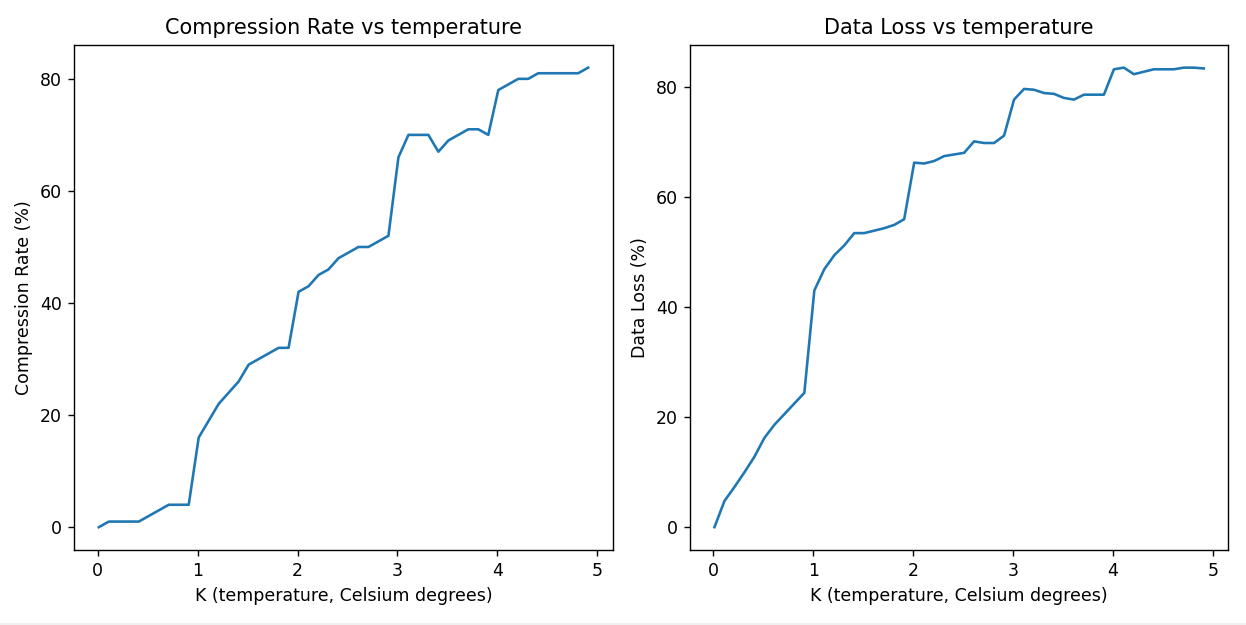
\includegraphics[width=1\textwidth]{krle_test.png}
    \caption{K-RLE результаты тестирования на датасете почасовой темперературы в Санкт-Петербурге в июне 2018 года}
    \label{fig:krle_test}
\end{figure}
Алгоритм K-RLE: Результаты показали, что коэффициент сжатия увеличивается с увеличением параметра K, но при этом также возрастает потеря данных. Графики показывают зависимость коэффициента сжатия и потери данных от параметра K.

Несмотря на высокий процент потерь данных, указанный на графике, высокий процент потери данных при сжатии не всегда является проблемой. В некоторых случаях допустимо иметь определенную степень погрешности для достижения значительного уменьшения объема данных, например при сборе метеорологических данных и при оптимизации энергопотребления сети Интернета Вещей.

\begin{figure}[ht]
    \centering
    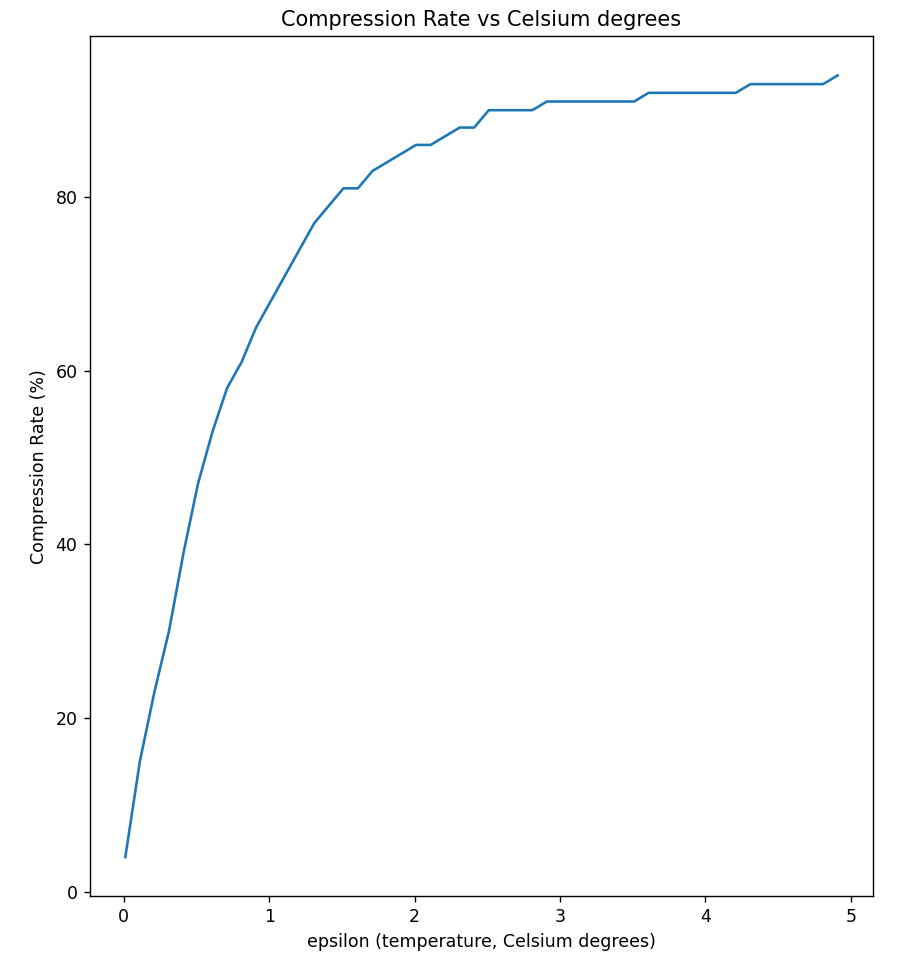
\includegraphics[width=1\textwidth]{ltc_test.png}
    \caption{LTC результаты тестрования на датасете почасовой темперературы в Санкт-Петербурге в июне 2018 года}
    \label{fig:ltc_test}
\end{figure}
Алгоритм LTC: Результаты показали, что коэффициент сжатия увеличивается с увеличением параметра $\epsilon$. График показывает зависимость коэффициента сжатия от параметра $\epsilon$. 

Графики наглядно демонстрируют компромисс между коэффициентом сжатия и потерей данных при использовании различных параметров для обоих алгоритмов.

\endinput